\documentclass[a4paper]{article}
\usepackage[left=2.1cm, right=2.1cm, top=2.1cm]{geometry}
\usepackage{lipsum}
\usepackage{tikzpagenodes}
\usepackage{pgfplots}
\usepackage{tikz}
\usepackage{tikz-3dplot}
\usetikzlibrary{arrows,decorations.pathmorphing,backgrounds,positioning,fit,matrix}
\pgfplotsset{compat=1.8}
\usepackage{graphics} % for pdf, bitmapped graphics files
\usepackage{epsfig} % for postscript graphics files
\usepackage[colorlinks=true,citecolor=green]{hyperref}
\usepackage{cite}
\usepackage{amsmath,amssymb,amsfonts}
\usepackage{algorithmic}
\usepackage{graphicx}
\usepackage{url}
\usepackage{cite}
\usepackage{bm}
\usepackage{pbox}
\usepackage{siunitx,booktabs,etoolbox}
\usepackage{ulem}
\usepackage[framed,numbered,autolinebreaks,useliterate]{mcode}
\usepackage{filecontents}
%\usepackage{bigfoot} % to allow verbatim in footnote


\def\BibTeX{{\rm B\kern-.05em{\sc i\kern-.025em b}\kern-.08em
    T\kern-.1667em\lower.7ex\hbox{E}\kern-.125emX}}

\begin{filecontents*}{ransac.m}
   clc;close all;clear all;

   [X, lineTrue] = gen_line_data(500);

   ph = tohomo(X);

   % your code starts here, do RANSAC line fitting
   params = xxxx(ph);
   
   % Results Visualization
   figure;
   hold on
   xmin = min(X(1,:));
   xmax = max(X(1,:));
   xx = linspace(xmin,xmax,100);
   yy1 = -(lineTrue(1).*xx+lineTrue(3))./(lineTrue(2)+1e-6);
   yy2 = -(params(1).*xx+params(3))./(params(2)+1e-6);
   plot(xx, yy1, 'k-.','LineWidth',1);
   plot(xx, yy2, 'm--','LineWidth',2);
   xlabel('x')
   ylabel('y')
   title('RANSAC results for 2D line estimation')
   axis equal tight
   set(gca,'FontName','Arial','FontSize',20);
\end{filecontents*}

\begin{document}

\title{Exercise on RANSAC}
%\author{xiahaa@space.dtu.dk}
\maketitle%%

In this exercise, you will work on line fitting using RANSAC.

\section{RANSAC}
Use the following code to generate simulated data for $2$D line fitting
\lstinputlisting{ransac.m}
Implement $4$ main routines for RANSAC: 
\begin{enumerate}
\item random sampling a minimum set.
\item estimating model parameters (\textbf{Hint: recall line fitting using homogeneous coordinate we did in the first exercise}).
\item compute consensus (\textbf{Hint: distance from point to line}).
\item update iteration.
\end{enumerate}
Result obtained:
\begin{figure*}[!b]
\centering
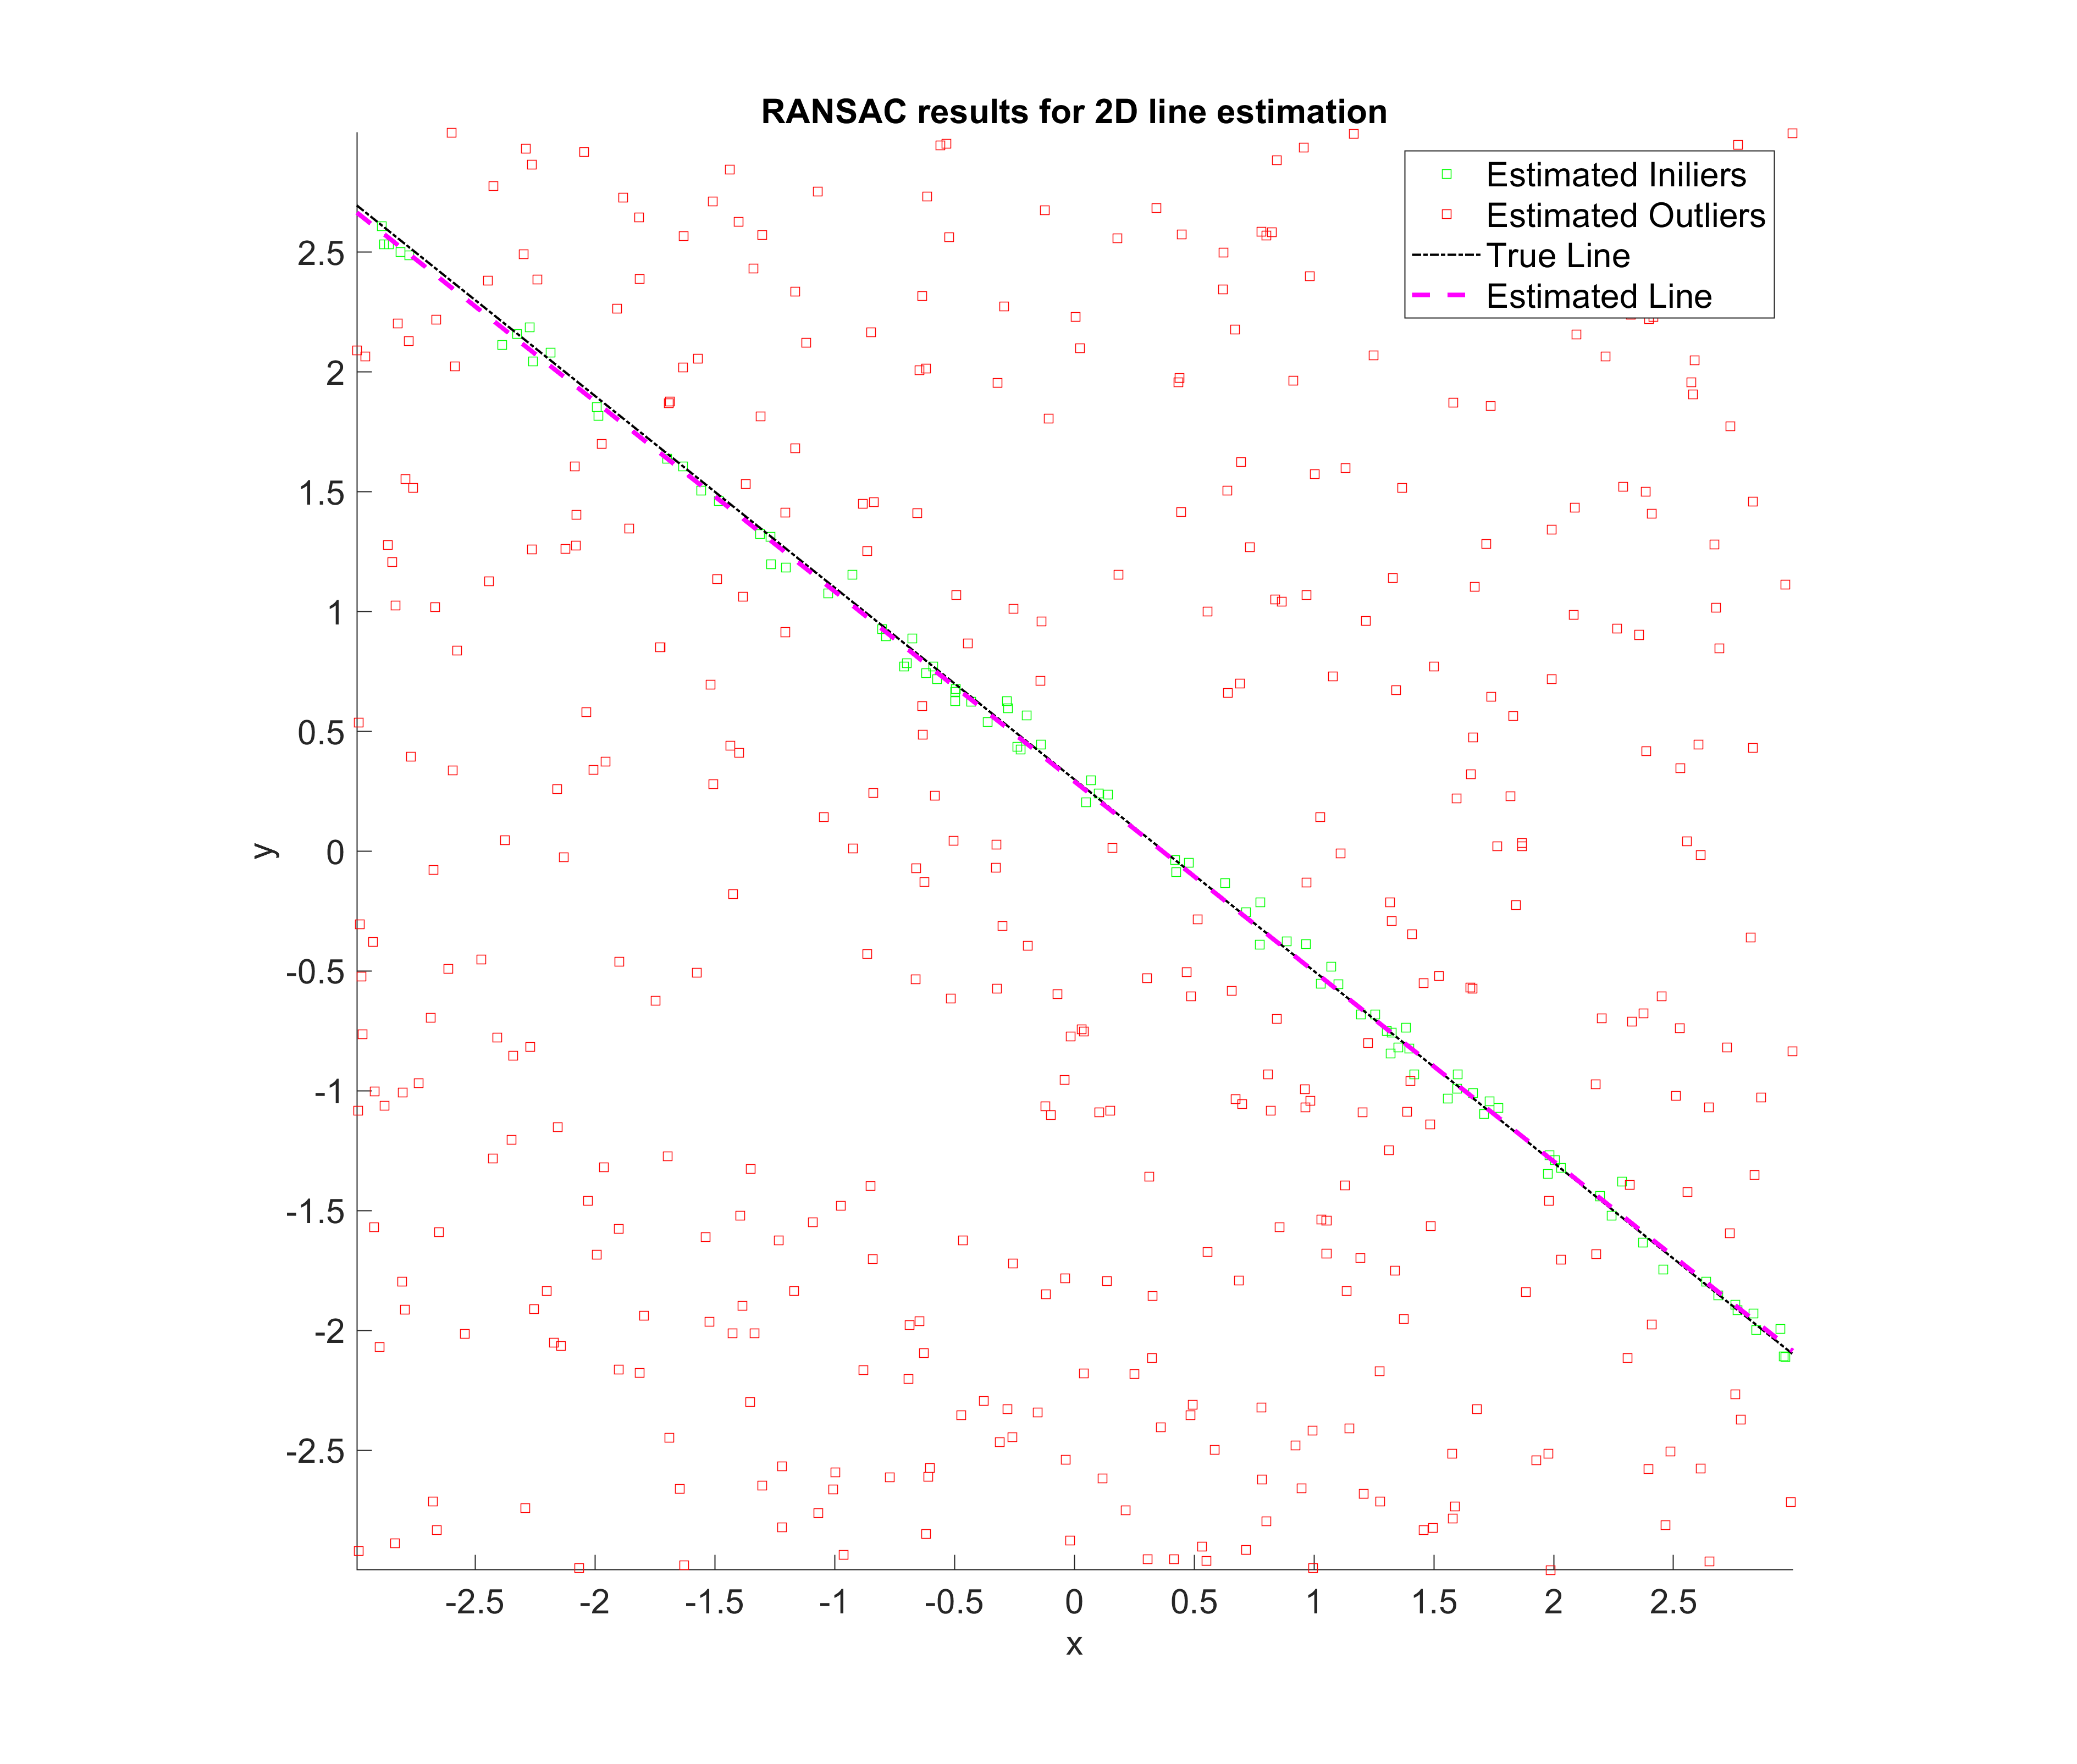
\includegraphics[scale=0.5]{figures/ransac.png}
\caption{Example of RANSAC line fitting.}
\end{figure*}

 
\bibliography{hand_eye_calibration} 
\bibliographystyle{ieeetr}

\end{document}